\chapter{Optimizing SNSPD HBT and TCSPC measurement of a fs laser source}


\section{Motivations and experimental setup overview}
\begin{figure}[hbtp]
\centering
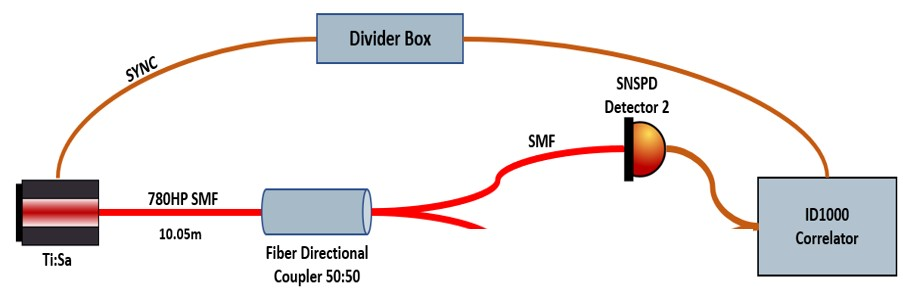
\includegraphics[width=1\textwidth]{TiSa_Setup.jpg}
\caption{Ciaone}
\label{TisaSetup}
\end{figure}



\section{Unwanted Side Peaks in HBT and TCSPC measurements}

\begin{figure}[hbtp]
\centering
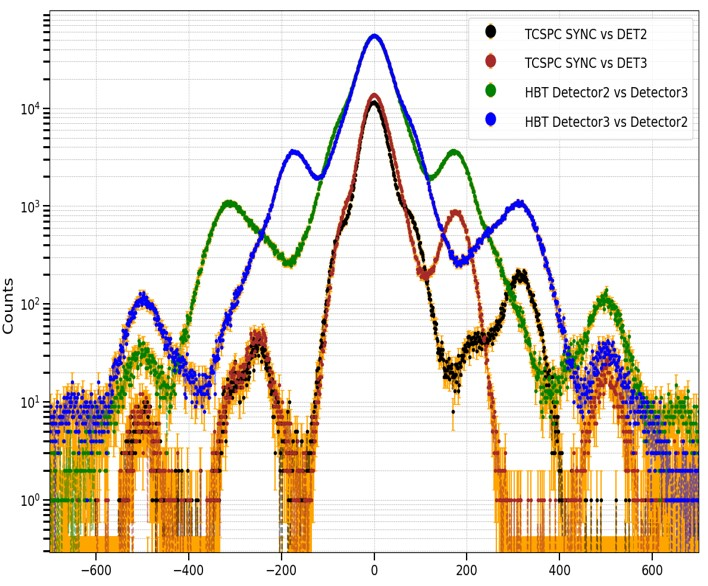
\includegraphics[width=1\textwidth]{Khaos.jpg}
\caption{Ciaone}
\label{Khaos}
\end{figure}
\section{Partly retrieving side peaks in HBT from coordinates of TCSPC peaks}

\begin{figure}[hbtp]
\centering
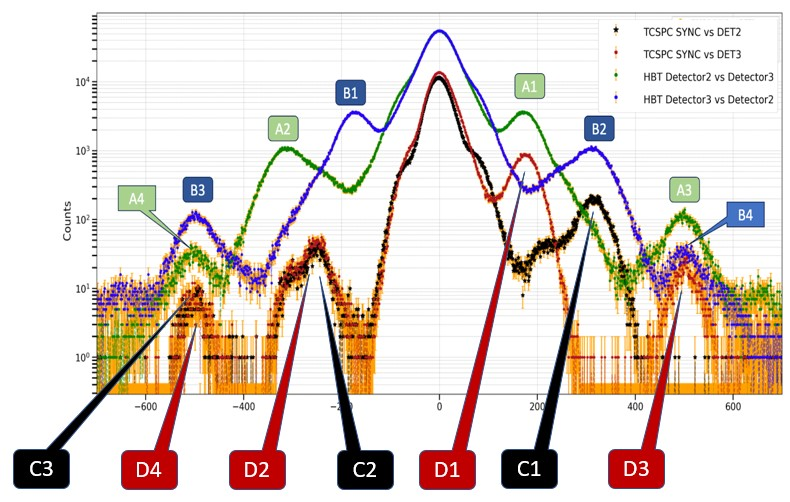
\includegraphics[width=1\textwidth]{Khaos_Labeled.jpg}
\caption{Ciaone}
\label{Khaos_labeled}
\end{figure}
\section{Measurements with improved detection thresholds}
\subsection{Driving idea}
\subsection{Discussion of the new measurements}
\subsection{Estimation of the width of the Detector response function}